\documentclass[12pt]{article}

\usepackage{amsmath}
\usepackage{amssymb}
\usepackage{amsthm}
\usepackage{hyperref}
\usepackage[pdftex]{graphicx}
%\usepackage{physymb}
\usepackage{wrapfig}
\usepackage{subcaption}
\title{EP 222: Assignment 1}

\author{Manish Goregaokar (120260006)}
\date{July 28, 2013}
\begin{document}
\maketitle
\section{Atwood's Machine}
\begin{figure}[h]
\centering
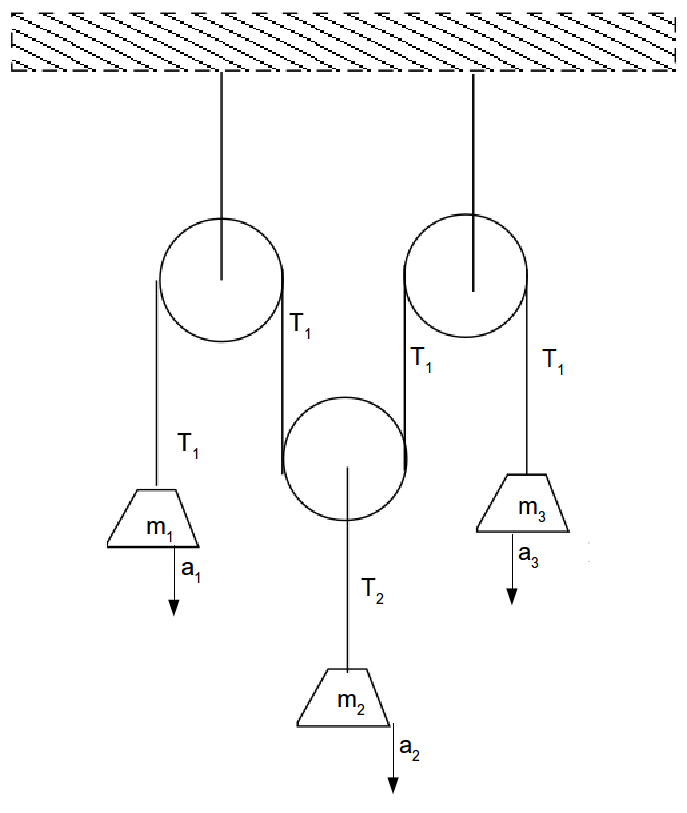
\includegraphics[scale=0.3]{AtD}
\caption{Diagram for Problem 1}

\label{fig:atd}
\end{figure}
 ~\\
\begin{wrapfigure}{r}{0.4\textwidth}
  \begin{center}
    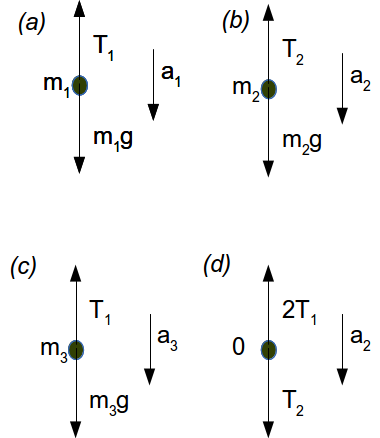
\includegraphics[width=0.38\textwidth]{atFBDs}
  \end{center}
  
  \caption{\footnotesize Free body diagrams: (a) For leftmost weight. (b) for middle weight. (c) For rightmost weight. (d) For middle pulley.}
  \label{fig:atfbds}
\end{wrapfigure}

I have defined the variables in Figure~\ref{fig:atd}.

Now, assuming that the pulleys are massless, and writing Newton's laws of motion for the central pulley, with FBD in Figure~\ref{fig:atfbds} (d), we get:

$$2T_1-T_2=0\times a_2=0$$ $$ \therefore T_2=2T_1$$

Now, if we assume that each block $m_i$ moves $x_i$ (downward positive) in a given time, the net work done by the strings will be $-(T_1x_1 + T_2x_2 + T_1x_3)$. This must be 0, as strings as a whole cannot do work. Differentiating twice with respect to time,\\~\\~\\ $$0=T_1\ddot x_1 + T_2\ddot x_2 + T_1\ddot x_3$$ $$\therefore T_1a_1 +2T_1a_2+T_1a_3=0$$ $$\therefore a_1 +2a_2 + a_3 =0$$

Now, applying Newton's second law on the other three FBDs, we get:

\begin{align}
T_1-m_1g &= m_1a_1\notag\\
2T_1-m_2g &= m_2a_2\notag\\
T_1-m_3g &= m_3a_3\notag
\end{align}

Firstly, let us substitute $a_i'=a_i+g $

This reduces our equations to 
\begin{align}
4g &= a_1' +2a_2' + a_3'\notag\\
T_1 &= m_1a_1'\notag\\
2T_1 &= m_2a_2'\notag\\
T_1 &= m_3a_3'\notag
\end{align}

Substituting values for $a_1',a_2',a_3'$ into the first equation, we get:

$$4g=\frac{T_1}{m_1} + 4\frac{T_1}{m_2} + \frac{T_1}{m_3}$$

$$\therefore T_1=\frac{4g}{\frac1{m_1}+\frac4{m_2}+\frac1{m_3}}=\frac{4gm_1m_2m_3}{m_1m_2+m_2m_3 + 4m_1m_3}$$

Substituting these values for $T_1$ back, we get:

\fbox{
 \addtolength{\linewidth}{-2\fboxsep}%
 \addtolength{\linewidth}{-2\fboxrule}%
\begin{minipage}{\linewidth}
\begin{align}
a_1 &=\frac{4gm_2m_3}{m_1m_2+m_2m_3 + 4m_1m_3} -g\notag\\
a_2 &=2\frac{4gm_1m_3}{m_1m_2+m_2m_3 + 4m_1m_3} -g\notag\\
a_3 &=\frac{4gm_1m_2}{m_1m_2+m_2m_3 + 4m_1m_3} -g\notag
\end{align}
\end{minipage}
}
\newpage
\section{Block system}
\begin{figure}[h]
\centering
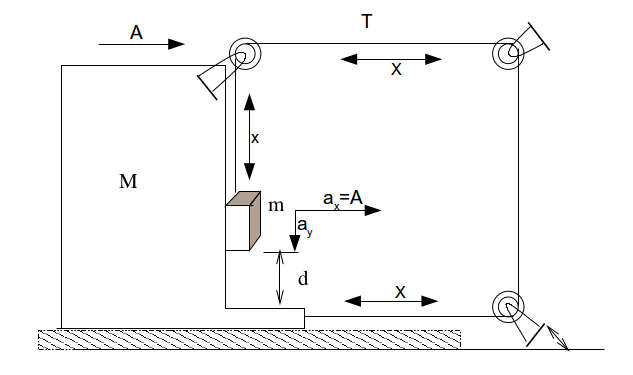
\includegraphics[scale=0.6]{2D}
\caption{Diagram for Problem 2}

\label{fig:2d}
\end{figure}

 ~\\
\begin{wrapfigure}{r}{0.4\textwidth}
  \begin{center}
    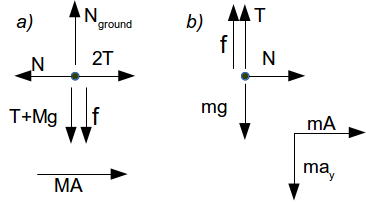
\includegraphics[width=0.38\textwidth]{2F}
  \end{center}
  
  \caption{\footnotesize Free body diagrams: (a) For large block $M$ (b) For small block $m$}
  \label{fig:2f}
\end{wrapfigure}

Let $a_x,a_y$ be the components of acceleration of the small block, and let $A$ be the acceleration of the large block.

Let $x$ denote the extension of the vertical string  and $X$ denote the contraction of the horizontal string where marked.

Now, if the block $M$ moves forward by $X$, the horizontal motion will "contract" these portions of the string by $2X$ (net change in length). This must be compensated for with the  expansion of the vertical portion of the string $x$, so $x=2X$ (as the total length of the string does not change, it is just redistributed). Differentiating, $\ddot x=2\ddot X\implies a_y=2A$.

Now, as the system is in motion, $f=\mu N$. Analyzing the horizontal direction with Newton's laws in Figure \ref{fig:2f} (a), we get: $$2T-N=MA$$

Analyzing Figure \ref{fig:2f} (b), we get: $$N=mA$$ $$mg-f-T=ma_y\implies mg-\mu N -T =ma_y$$


Substituting $N=mA$ and $a_y=2A$, we get:

$$2T=(m+M)A$$

$$mg-\mu mA -T=2mA$$

Solving, we get $$A=\frac{2g}{5+2\mu+\frac Mm}$$

This implies  $$a_y=\frac{4g}{5+2\mu+\frac Mm}$$

Substituting $\frac Mm=10, \mu=0.5$, we get:

$$A=a_x=\frac14 g, a_y=\frac12 g$$

Thus vector acceleration of $M$ is \fbox{$\frac14g \hat i $}, acceleration of $m$ is \fbox{$\frac14g(\hat i -2\hat j) $}

As initual downward velocity of $m$ is 0, time taken to cover a distance of $d=2.45 ~\mathrm m$ is $\sqrt{\frac{2d}{a_y}}$ (from $s=ut+\frac12 at^2$), which is $\sqrt{\frac{4.9}{9.8\times \frac{1}{4}}} = \sqrt{2}~\mathrm s$

Thus the block takes \fbox{$1.414$ seconds} to reach the bottom.
\newpage
\section{Rod on belt}
\begin{figure}[h]
\centering
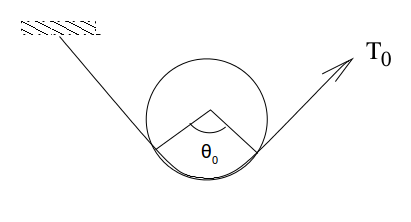
\includegraphics[scale=0.6]{3D}
\caption{Diagram for Problem 3}

\label{fig:3d}
\end{figure}
 ~\\
\begin{wrapfigure}{r}{0.3\textwidth}
  \begin{center}
    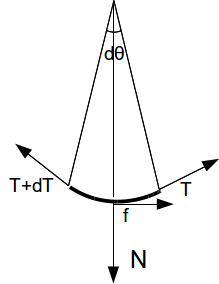
\includegraphics[width=0.38\textwidth]{3D2}
  \end{center}
  
  \caption{\footnotesize Close up of small element of rope}
  \label{fig:3D2}
\end{wrapfigure}

Let us analyze a small portion of the belt, as tension on that belt is changing. We assume that friction acts to the right.

Now, the horizontal component of tension is $(T+dT-T)\cos{\frac12 d\theta}=dT$. The vertical component is $(T+T+dT)\sin{\frac12 d\theta}=Td\theta$.

Balancing forces, we get $N=Td\theta$, and $f=dT$. Now, $f\leq \mu N \implies dT\leq \mu Td\theta$.

Integrating, $\int\limits_{T_0}^T \frac{dT}{T}=\int\limits_0^\theta \mu d\theta$. From here, we get that 

$T(\theta)\leq T_0e^{\mu\theta}\implies T_{wall}\leq T_0e^{\mu\theta_0}$

If we assume that friction acts to the left, we get $T_{wall}\geq T_0e^{-\mu\theta_0}$

Now, the macroscopic variable $T_{wall}$ depends on the microscopic distribution of elongation in the string, which in turn depends on the process used to create this system. This is an unknown, which gives us a range (instead of an absolute answer) for $T_{wall}$ However, Newton's laws allow all values of $T_{wall}$ between $T_0e^{-\mu\theta_0}$ and $T_0e^{\mu\theta_0}$. Thus, we can claim that a state can be constructed where \fbox{$T_{wall}=T_0e^{\mu\theta_0}$}, and this is the maximum tension possible.

\section{Leaning ladder}
\begin{figure}[h]
\centering
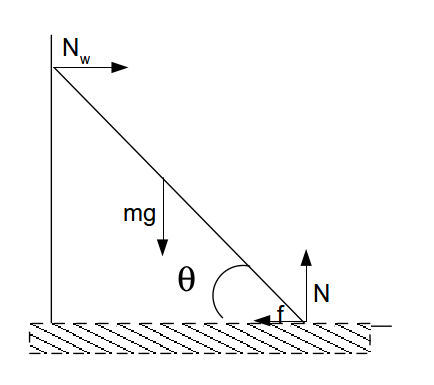
\includegraphics[scale=0.6]{4D}
\caption{Diagram for Problem 4}

\label{fig:4d}
\end{figure}

Firstly, let us assume that the ladder has a length $2L$ and mass $m$. 

Now, note that the smallest angle in equilibrium will be  when the static friction attains its maximum value ($\mu N$). So, $f=\mu N$.

Now, first writing translational equilibrium equations:

$$mg=N$$
$$\mu N=f = N_w$$

The net torque on the ladder is $\tau=N_wL\sin\theta+fL\sin\theta - NL\cos\theta$. The ladder is in rotational equilibrium, so $\tau=0$. So, $$N_w L\sin\theta +fL\sin\theta =NL\cos\theta$$

Making substitutions from previously derived equations, we get $$2\mu NL\sin\theta=\cos\theta$$

or $$\boxed{\theta=\cot^{-1}2\mu}$$

\section{Cylinders}

\begin{figure}[h]
\centering
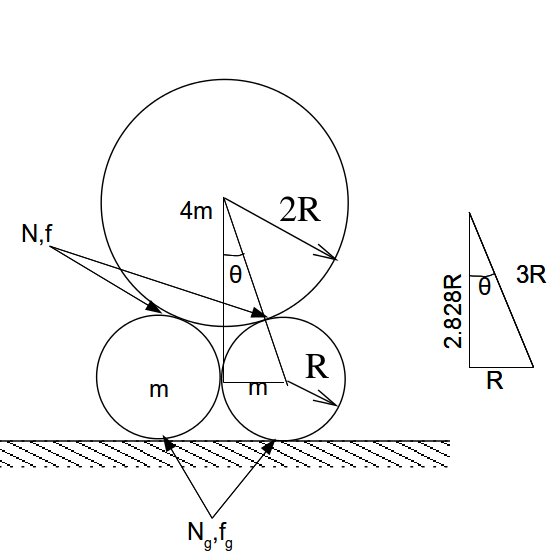
\includegraphics[scale=0.4]{5D}
\caption{Diagram for Problem 5}

\label{fig:5d}
\end{figure}
 


Here, we assume that there is friction between the small cylinders and the large one, as otherwise we get that the system does not stay in rotational equilibrium. This is easily verified, as the only forces providing torque to the smaller cylinders are the friction from the ground and the friction between them and the larger cylinder.\\  As the grund friction is nonzero, there must be friction between the smaller cylinders and the larger one otherwise the system does not stay at rest. Note that the friction between the cylinders must be zero due to the symmetry of the system.\\

The free body diagrams have been labelled taking into account the symmetry of the system. Figure \ref{fig:5d} indicates the contact forces at various points (direction is not shown as it  depends on which body we are considering, refer Figure \ref{fig:5f} for details on the direction of the forces).
\begin{wrapfigure}{l}{0.5\textwidth}
  \begin{center}
    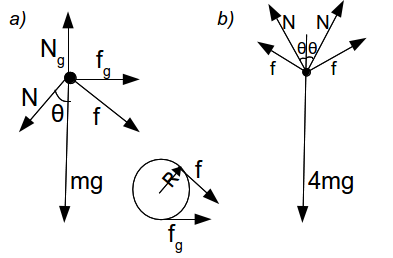
\includegraphics[width=0.38\textwidth]{5F}
  \end{center}
  
  \caption{\footnotesize Free body diagrams: (a) For small cylinders $(m,R)$ (b) For large cylinder $(4m,2R)$}
  \label{fig:5f}
\end{wrapfigure} 
Now, we first write the equation for torational equilibrium for the small cylinders, $\tau=rf_g-rf=0 \implies f_g=f$. We can thus conveniently replace all $f_g$ with $f$.

Writing the equations for translational equilibrium of the small cylinders, we get

\newcommand{\ccc}{\cos\theta}
\newcommand{\sss}{\sin\theta}

$$mg + N\ccc +f\sss = N_g$$

$$N\sss =f+f\ccc$$

Writing equilibrium equations in the vertical direction for the large cylinder:

$$2N\ccc+2f\sss=4mg\implies N\ccc +f\sss=2mg$$

Note that $\theta$ is known, with $\sss=\frac13, \ccc=\frac{\sqrt8}3$

$$\therefore N=f(1+\sqrt8)$$
$$N\sqrt 8 +f=6mg$$
$$\therefore f(1+\sqrt 8) + f =6mg\implies f=\frac{6mg}{2+\sqrt 8}$$

$$\therefore N=6mg\frac{1+\sqrt8}{2+\sqrt8}$$

As $$Ng=mg + N\ccc +f\sss $$
\begin{align}
N_g &= mg + 6mg\ccc\frac{1+\sqrt8}{2+\sqrt8} + \sss\frac{6mg}{2+\sqrt 8}\notag\\
 &= mg \left(1 + \frac{6}{3(2+\sqrt 8)}\left(\sqrt8(1+\sqrt8) + (2+\sqrt8)\right) \right)\notag\\
 &= mg\left(1+\frac{1}{1+\sqrt 2}\left(10+4\sqrt2\right)\right )\notag\\ 
 &=mg\frac{11+5\sqrt 2}{1+\sqrt 2}\notag
\end{align}

$$\therefore \frac{N_g}{f_g}=\frac{\left(mg\frac{11+5\sqrt 2}{1+\sqrt 2}\right)}{\left(\frac{3mg}{1+\sqrt 2}\right)}=\frac{11+5\sqrt 2}{3}$$

Now, $\mu N_g\geq f_g$. In this case, the minimum $\mu$ is during equality, so \fbox{$\mu=\frac{N_g}{f_g}= \frac{11+5\sqrt 2}{3}$}

\section{Mass on wedge}
\begin{figure}[h]
\centering
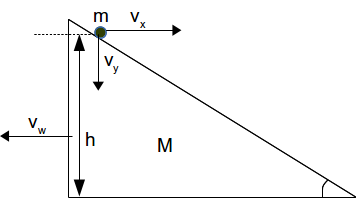
\includegraphics[scale=0.4]{6D}
\caption{Diagram for Problem 6}

\label{fig:6d}
\end{figure}

Here, I am assuming that the values of final velocity are required just before the mass $m$ reaches the table (as to calculate this value at the exact time will require knowledge of the nature of the collision). For the purposes of this problem I shall take the symbols $v_w,v_x,v_y$ to mean the velocities at the final stage. Initial velocities are zero.

Now, we can conserve momentum in the horizontal direction here and overall energy as well. Conserving momentum in the horizontal direction, we get $mv_x=Mv_w \implies v_x=\frac Mm v_w$.

Conserving energy, $\frac12(Mv_w^2+mv_x^2+mv_y^2)=mgh$

Finally, in the wedge frame, the mass must move along the wedge surface. Thus, $\frac{v_y}{v_x+v_w}=\tan\theta \implies v_y=\tan\theta (v_x+v_w)$

Substituting the values for $v_x$ and $v_y$ in the energy conservation equation, we get 

$$2mgh= Mv_w^2+ m\left(\frac{M}m v_w\right)^2+m\tan^2\theta (v_x+v_w)^2=Mv_w^2+ m\left(\frac{M}m v_w\right)^2+m\tan^2\theta v_w^2 \left(1+\frac{M}{m}\right)^2$$


$$\therefore v_w^2 = \frac{2mgh}{M+\frac{M^2}{m} + m\tan^2\theta \left(1+\frac{M}m\right)^2}$$

$$\therefore \boxed{v_w=\sqrt{\frac{2mgh}{M+\frac{M^2}{m} + m\tan^2\theta \left(1+\frac{M}m\right)^2}}}$$

\end{document}